\vsssub
\subsubsection{~$S_{ref}$：岸线和冰山处的能量反射} \label{sec:REF1}
\vsssub

\opthead{REF1}{\ws}{F. Ardhuin}

\noindent 
岸线和冰山反射通过使用 {\code REF1} 开关，并把 namelist 参数 {\code REFCOAST}、{\code REFSUBGRID} 或 {\code REFBERG}（在 {\F REF1} namelist 中）设为非零值来激活；这些非零值是波能目标反射系数 $R_0^2$。如果同时使用 {\code IG1} 开关，则岸线处的能量源还包括入射和出射两个方向上的自由次重力波。该特定源项见第 \ref{sec:IG1} 节。

由这些值给出的 $R_0^2$ 可按照 Miche 型参数随波高和周期变化：这通过把 {\code REFFREQ} 设为非零值激活，并基于 \cite{art:EHG94} 的现场测量。这些系数也可通过把 {\code REFMAP} 设为非零值而具有空间变化。在这种情况下，ww3\_grid 会在 ww3\_grid.inp 中读取水深和阻挡之后，预期再读入一行额外内容，用来定义岸线坡度图。该图中的值会乘以 {\code REFMAP} 的值。

岸线处的波浪反射可从入射波能的百分之几到约 50\% 不等，并可能对方向波谱以及原本受遮蔽位置的波候产生重要影响 \citep{pro:ORe99}。波浪反射对于海洋波浪产生地震噪声也极为重要。

由于反射涉及不同方向的波列，在 \ws\ 这样的模式中，它们的相互作用只能通过右端源项表示。不过，这一过程在物理上与传播相联系。

在实际处理中，对于规则网格和曲线网格，反射源项把适量能量放入反射波方向；这些能量将在下一时间步由传播项移除。忽略横岸流时，有

\begin{equation} 
\cS_{ref}(k,\theta) = 
\int R^2(k,\theta,\theta') \frac{C_g(k)}{\Delta A} \left[\cos (\theta-\theta_q) \Delta q + \sin (\theta-\theta_p)  \Delta p \right] N(k,\theta') \mathrm{d} \theta' \; ,
\end{equation}

\noindent
其中 $R^2$ 为能量反射系数，$\Delta p$ 和 $\Delta q$ 分别为沿网格两个轴向的网格距，$\Delta A$ 为单元面积。如何从陆海掩膜定义岸线方向见 \cite{art:Aea11}。这尚未在 SMC 网格上测试，也不预期适用于该类型网格。

对于非结构网格，边界处出射方向的谱密度直接设为预期反射值，边界条件由数值格式专门处理。


反射系数 $R^2$ 仅在满足 $\cos(\theta-\theta')<0$ 的方向上取非零；其大小为在散射方向 $\theta$ 上积分的反射系数 $R_0^2(k)$ 与围绕镜面反射方向 $\theta_s$ 的方向分布 $R_2(\theta,\theta')$ 的乘积：

\begin{equation} 
R^2(k,\theta,\theta')  =  R_0^2(k) R_2(\theta,\theta') \:\:\: .
\end{equation}

\noindent
该方向分布有三种形式：
\begin{itemize}

\item 在所有与入射方向相反的方向上各向同性：用于子网格岛屿、冰山或尖锐岸线角；

\item 对中等岸线角，正比于 $\cos(\theta-\theta_s)^2$；

\item 对较小岸线角（近乎笔直的岸线），正比于 $\cos(\theta-\theta_s)^n$。默认 $n=4$，可使用 {\F REF1} namelist 中的 {\code REFCOSP\_STRAIGHT} namelist 参数改为任意值。

\end{itemize}

\noindent
该参数化由 \cite{art:AR12} 详细说明。

对于冰山和子网格岛屿，反射能量在与入射波相反方向夹角 90$\degree$ 以内的所有方向上均匀再分配。对于已解析陆地，则由局地点周围 8 个网格点的陆地或海洋状态定义垂直于岸线的平均方向 $\theta_n$（图 \ref{fig:refl}）。

对每个邻近陆地的模式网格点，陆海几何分析会在 16 个可能方向中给出一个 $\theta_n$ 值。它与任一入射波方向 $\theta_i$ 一起定义镜面反射方向 $\theta_r=2 \theta_n - \theta_i + \pi$。对于朝向海岸的方向 $\theta_i$ 的每个谱分量（即满足 $\cos(\theta_i-\theta_n) >0$），总反射为入射能量的 $R^2$ 倍。该反射能量 $R^2 E(f) M(f,\theta_i)$ 在镜面反射方向 $\theta_r$ 附近的方向上再分配，采用宽方向分布，正比于 $\cos^n(\theta-\theta_r)$，其中幂次 $n$ 是局地岸线几何的函数。

\begin{figure} \begin{center}
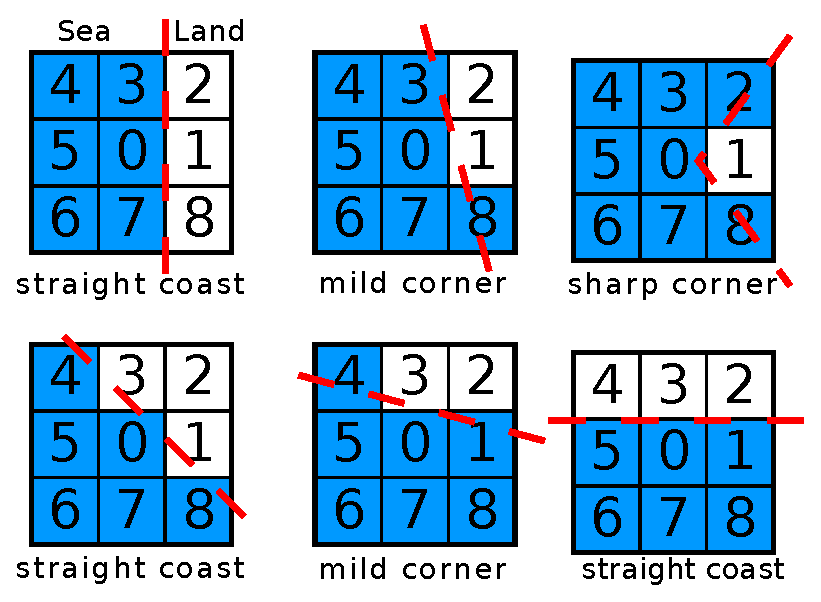
\epsfig{file=./num/coast_reflection.eps,angle=0,width=3in}
\caption{使用陆海掩膜确定岸线取向和几何的示例。对于任一海点（编号 0，蓝色海洋）且其至少有一个邻点为陆地（白色），使用编号为 1 到 8 的八个相邻点定义岸线几何。对于“平缓”拐角和笔直海岸，估计的岸线取向（虚线）用于计算反射波能的方向分布。}
\label{fig:refl} \botline
\end{center}
\end{figure}

为此，我们按图 \ref{fig:refl} 所示区分相对于局地点的三种岸线几何：对笔直海岸（相邻点中有三个连通陆点）设 $n=2$；对平缓拐角（相邻点中有两个陆点）设 $n=1$；对尖锐拐角（4 个最近相邻点中仅有一个陆点）设 $n=0$，这对应与子网格岛屿和冰山相同的处理。把这些 $n$ 值在 $0$ 到 $2$ 范围内改变，对结果影响很小。$n=1$ 对应 Lambert 面近似，该近似用于粗糙表面的电磁波散射。若 $n$ 为无穷大，则得到纯镜面反射。更严格的处理应使用海洋波长尺度上的岸线取向分布，即约 100~m 量级。
